\documentclass[dvipdfmx]{standalone}% ドライバ dvipdfmx を指定する
\usepackage{tikz}
\usetikzlibrary{shapes, arrows.meta, positioning, shapes.geometric}

\begin{document}

%\begin{tikzpicture}[paint/.style={draw=#1!75, fill=#1!20}]
%  \tikzset{every node/.style={isosceles triangle, draw, inner sep=0pt,
%    anchor=left corner, shape border rotate=90}}
%  \draw[help lines] grid(4,2);
%  \foreach \a/\c in {1.5/blue, 1/green, 0.5/red}{
%    \node[paint=\c, minimum height=\a cm] at (1,0) {};
%    \node[paint=\c, minimum width=\a cm] at (3,0) {};
%  }
%\end{tikzpicture}


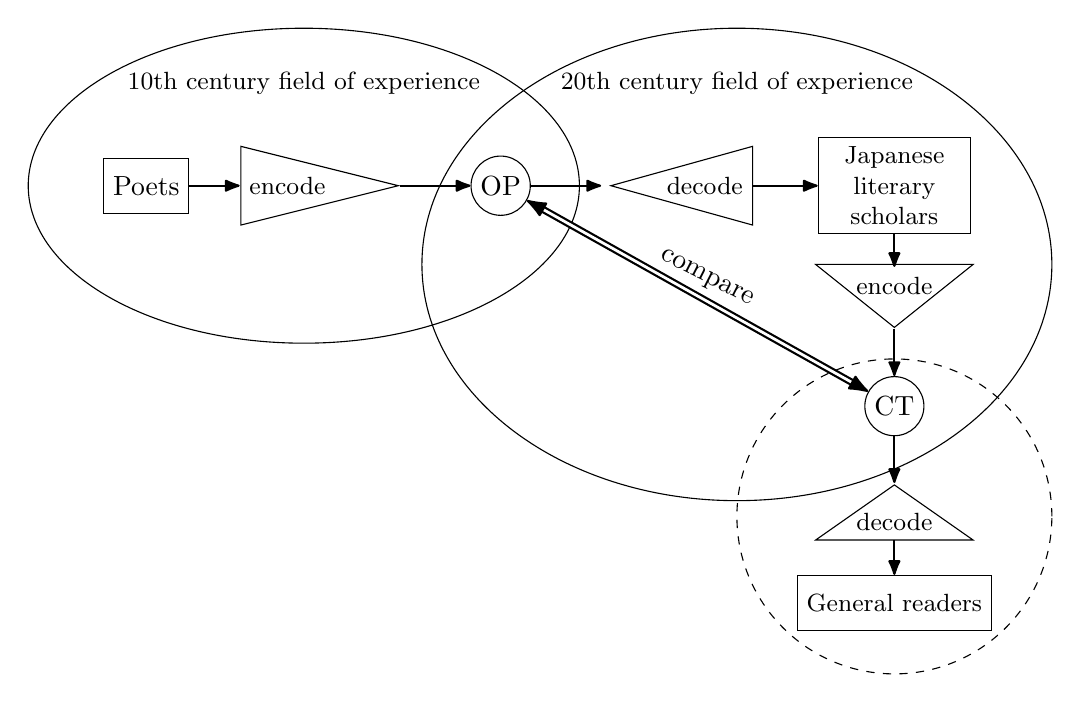
\begin{tikzpicture}[
 % node distance = 1cm and 1cm and 1cm and 1cm, 
%     every node/.style={draw, font=\small, align=center},
    circle node/.style={circle, draw, minimum size=.7cm, inner sep=0.7mm},
    rect node/.style={rectangle, draw, minimum width=0.5cm, minimum height=.7cm},
    arrow/.style={->, thick, >=Latex[round]},
    double arrow/.style={<->, thick, double, double distance=1pt,>=Latex[round]}
    ]

    
    % 三角形のパスを定義

%    \draw [help lines] (0,0) grid (15,10);%(0,0)から(10,4)までの"細線の方眼"

    % 10世紀のノード

%\node[isosceles triangle, draw, minimum height = .5cm, minimum width =2cm] (T30)at (6,6){};

    \node[ellipse, draw, minimum width=7cm, minimum height=4cm] (Z1) at (4.5,7) {};
    \node at (4.5, 8.3) {\small 10th century field of experience};

    \node[rect node] (POET) at (2.5,7) {Poets};

    \draw (3.7,7.5) -- (5.7,7) -- (3.7,6.5) -- cycle;
    \node[left] (T1s) at (4.9, 7) {\small encode};
    \node (T1e) at (5.6, 7) {};

    \node[circle node] (OP) at (7,7) {OP};


    % 20世紀のノード
    \node[ellipse, draw, minimum width=8cm, minimum height=6.0cm] (Z2) at (10,6.0) {};
    \node at (10, 8.3){\small 20th century field of experience}; 

    \draw (10.2,7.5) -- (8.4,7) -- (10.2,6.5) -- cycle;
    \node (T2s) at (8.4, 7) {};
    \node[left] (T2e) at (10.2, 7) {\small decode};

    \node[rect node] (JLS) at (12.0,7) {
        \begin{minipage}[c]{1.7cm}
          \small
          \centering
            Japanese \\literary\\ scholars
          \end{minipage}
    };

    \draw (11.0,6.0) -- (13.0,6) -- (12.0,5.2) -- cycle;
    \node[above](T3s) at (12.0, 5.5) {\small encode};
    \node (T3e) at (12.0, 5.3) {};

    \node[circle node] (CT) at (12,4.2) {CT};

    \draw (11.0,2.5) -- (13.0,2.5) -- (12.0,3.2) -- cycle;
    \node(T4s) at (12.0, 3.1) {};
    \node[above] (T4e) at (12.0, 2.5) {\small decode};


    \node[ellipse, draw, dashed, minimum width=4.0cm, minimum height=4.0cm] (Z1) at (12.0,2.8) {};
    \node[rect node] (GR) at (12.0,1.7) {\small\centering General readers};

    % 矢印
    \draw[arrow] (POET) -- (T1s);
    \draw[arrow] (T1e) -- (OP);
    \draw[arrow] (OP) -- (T2s);
    \draw[arrow] (T2e) -- (JLS);
    \draw[arrow] (JLS) -- (T3s);
    \draw[arrow] (T3e) -- (CT);
    \draw[arrow] (CT) -- (T4s);
    \draw[arrow] (T4e) -- (GR);

    % 比較の矢印
    \draw[double arrow,>={Latex[round]}] (OP) -- (CT) node[midway, above, rotate=-27] {compare};

\end{tikzpicture}

\end{document}
